\documentclass{beamer}
\usepackage{amsfonts,amsmath,oldgerm}
\usepackage{hyperref}
\usetheme{sintef}

\newcommand{\testcolor}[1]{\colorbox{#1}{\textcolor{#1}{test}}~\texttt{#1}}

\usefonttheme[onlymath]{serif}

\titlebackground*{assets/background}

\newcommand{\hrefcol}[2]{\textcolor{cyan}{\href{#1}{#2}}}

\title{Politecnico di Torino}

% Added vspace commands to adjust the distance between title, subtitle, and group members
\subtitle{\vspace{10pt} Assignment 1 of the course \\ Information Theory for Data Science \vspace{6pt}}

\author{
    {\LARGE \textbf{Group Members:}} \\[8pt]  % Increased size and added more spacing
    {\normalsize Alessandro Conforti (s346511)} \\[6pt]    % Made the names smaller and adjusted spacing
    {\normalsize Alessandro Maini (s3346219)} \\[6pt]
    {\normalsize Ali BehlooeiDolatsaraei (Student Number)} \\[6pt]
    {\normalsize Sina Behnam (Student Number)} \\[6pt]
    {\normalsize Hojjat Miryavifard (s334026)}
}

\date{October 8, 2024}




\begin{document}
\maketitle

\begin{frame}

In this report, we are going to solve the following exercises:

\textbf{Exercises:}

1. Entropy of a random variable with 3 outcomes (pt. 3)

2. Entropy of a random variable from a data series (pt. 4)

3. Application of the principle of maximum entropy (pt. 4)

4. Exercise on Information Gain Ratio (pt. 4)

5. Kullback-Leibler divergence from empirical distribution (pt. 3)

6. Permutation entropy for anomaly detection (pt. 5)

7. Information Gain Ratio and Classifier (pt. 7) (not yet available)

\end{frame}


% Include exercise1.tex
\section{Exercise 1: Entropy of a Random Variable with 3 Outcomes}

\begin{frame}{Entropy and Probability Vectors}
In this exercise, we analyzed the entropy of a random variable with three possible outcomes. The entropy \( H(p) \) is defined as:

\[
H(p) = - \sum_{i=1}^3 p_i \log_2 p_i
\]

where \( p = [p_1, p_2, p_3] \) represents the probability vector for the outcomes. The goal was to:
\begin{itemize}
    \item Calculate entropy over the probability simplex.
    \item Apply an iterative averaging procedure to observe entropy evolution toward uniformity.
    \item Show that entropy approaches its maximum as the distribution becomes uniform.
\end{itemize}
\end{frame}

\begin{frame}{Entropy over the Probability Simplex}
We generated all valid probability vectors where \( p_1 + p_2 + p_3 = 1 \) and \( p_i \geq 0 \), and computed the entropy for each. The highest entropy occurs when the probabilities are equally distributed (\( p_1 = p_2 = p_3 \)).

\vspace{3mm}  % Add vertical space between the text and the graph

\begin{figure}[ht]
    \centering
    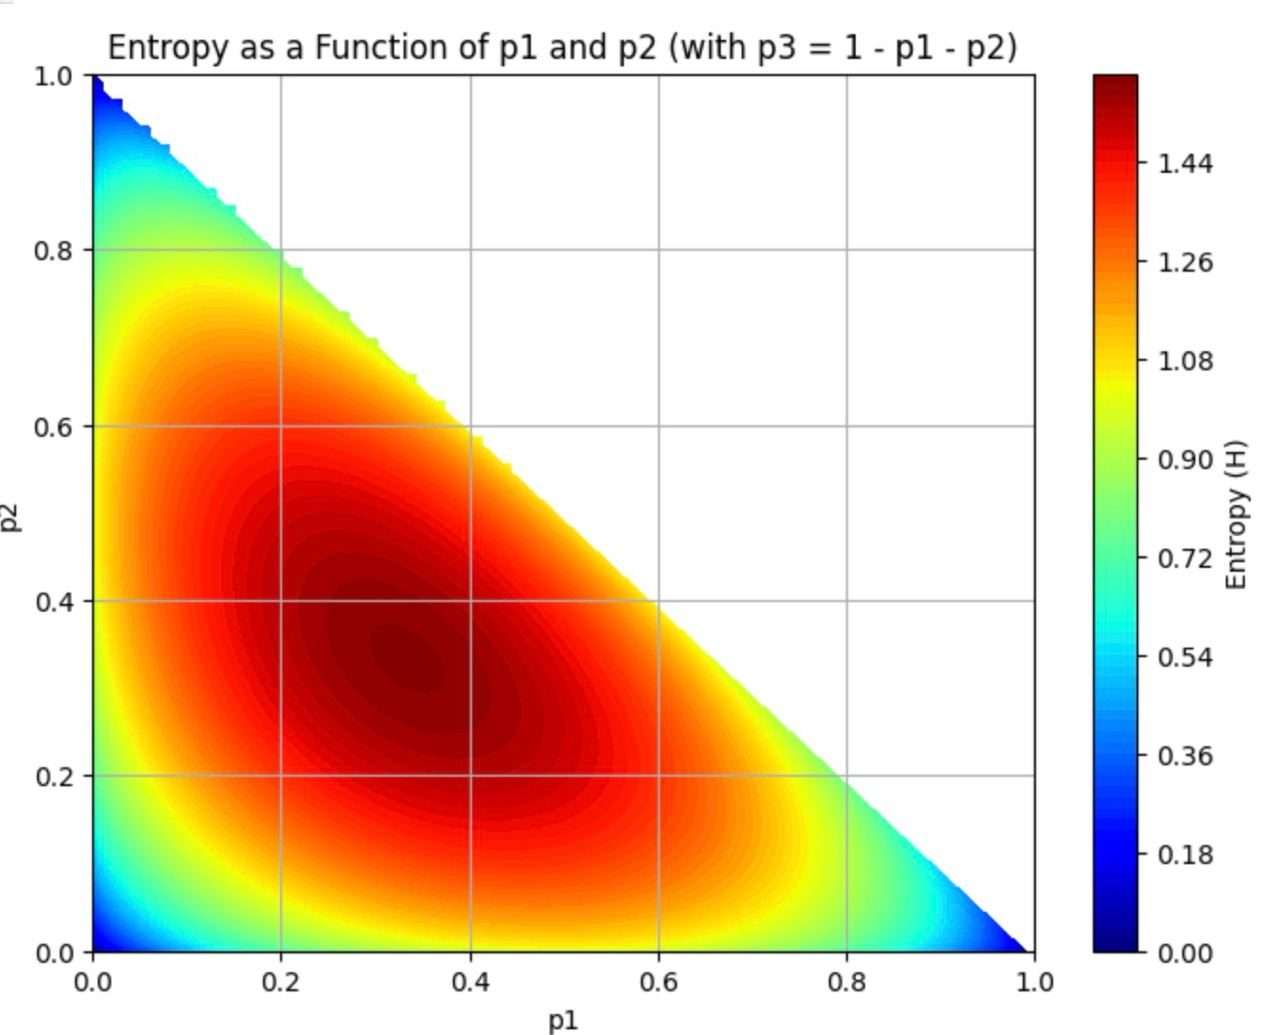
\includegraphics[width=0.4\textwidth]{images/2.jpg}
    \hspace{5mm}
    \parbox[b]{0.3\textwidth}{\caption{Figure 1: Entropy across the probability simplex. Highest entropy at uniform distribution.}}  % Correct the double "Figure" issue
    \vspace{-5mm}  % Bring the caption closer to the graph
\end{figure}
\end{frame}


\begin{frame}{Iterative Averaging Procedure}
We started with a skewed probability vector \( p = [0.98, 0.01, 0.01] \) and applied an iterative averaging procedure. Probabilities were updated and normalized after each iteration, demonstrating how the distribution evolves towards uniformity.

\vspace{3mm}  % Add vertical space between the text and the graph

\begin{figure}[ht]
    \centering
    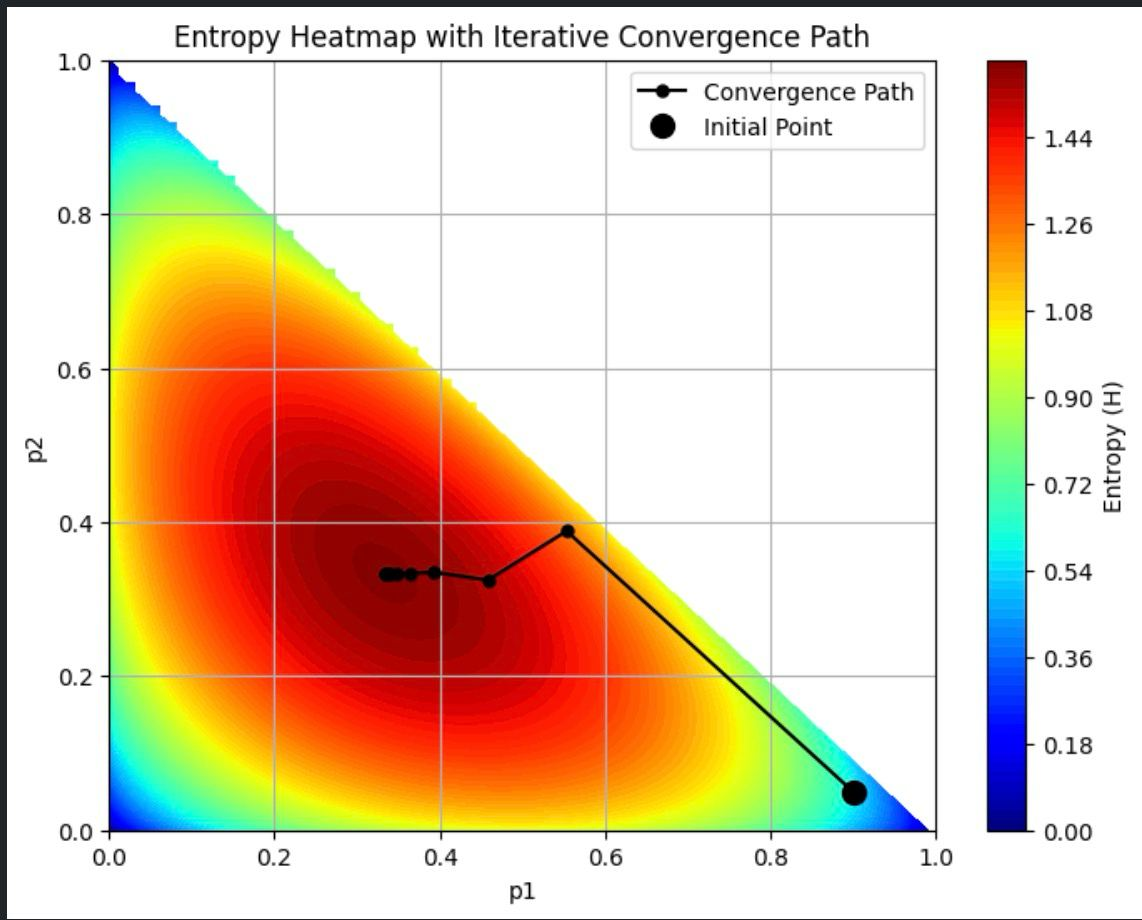
\includegraphics[width=0.4\textwidth]{images/1.jpg}
    \hspace{5mm}
    \parbox[b]{0.3\textwidth}{\caption{Figure 2: Entropy evolution during iterative averaging. Entropy rises as the distribution balances.}}  % Correct the double "Figure" issue
    \vspace{-5mm}  % Bring the caption closer to the graph
\end{figure}
\end{frame}

\begin{frame}{Results and Conclusion}
In this exercise, we:
\begin{itemize}
    \item Calculated entropy over the probability simplex, confirming that entropy is maximized when probabilities are uniformly distributed.
    \item Applied an iterative averaging process starting with a skewed probability vector. Each iteration brought the distribution closer to uniformity, with the corresponding entropy values increasing, approaching the theoretical maximum.
    \item Visualized the convergence of the entropy values as the probability vector approached uniformity.
\end{itemize}

Overall, the experiment demonstrated the direct relationship between entropy and distribution balance: skewed distributions have low entropy, while uniform distributions achieve maximum entropy. The iterative procedure successfully illustrated how entropy evolves as randomness in the distribution increases.
\end{frame}


\section{Exercise 2: Entropy of a random variable from a data series}

\begin{frame}{ Entropy of a random variable from a data series}

In this exercise, our aim is to:
\begin{itemize}
    \item Identify a data series and estimate the probabilities of the outcomes based on
their occurrences, updating the probabilities at each time step.
    \item At each time step, compute the entropy, plot its behaviour, and discuss the results
\end{itemize}
\end{frame}


\begin{frame}{Data Series Overview}
This dataset could be very suitable for our entropy calculation exercise, as it provides a real-world time series that likely exhibits interesting patterns and variations over time. The data is organized as a time series, meaning it's collected at regular time intervals (daily in this case) over a while. We have used Delhi's temperature record for over 4 years.
This is the\href{https://www.kaggle.com/datasets/sumanthvrao/daily-climate-time-series-data}{"link"} to the dataset.

Although the dataset contains other information like date, mean temperature, humidity, wind speed, and mean pressure, we mainly focused on mean temperature and dropped all the rest.
\end{frame}

\begin{frame}{Data Distribution}
The distribution below represents temperature data distribution which shows the frequency of bins, each bar represents a 2°C temperature range, as specified in the code
\begin{figure}
    \centering
    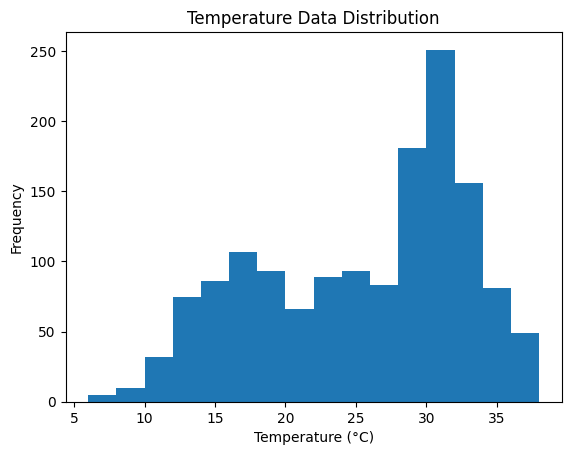
\includegraphics[width=0.5\linewidth]{temp_distribution.png}
    \label{fig:enter-label}
\end{figure}
\end{frame}
\begin{frame}{Probability Estimation}
Binning is necessary to transform continuous temperature data into discrete categories, making it possible to compute the probabilities of the temperature falling within specific ranges. Once the data is binned, the frequency of data points in each bin is counted. These frequencies are then converted into probabilities by dividing each count by the total number of data points at each time step.
These probabilities represent the likelihood of the temperature falling within each bin at a given time. using Shannon’s entropy formula, entropy is computed for each time step based on the probabilities of the data falling within different bins.


Entropy $H(X)$ is calculated based on the following formula derived from Shannon’s work:
\[
H(X) = -\sum_{i=1}^{n} p(x_i) \log_2{p(x_i)}
\]
\end{frame}

\begin{frame}{Iterative Calculation Over Time}
The core of the code involves a loop that recalculates entropy as the dataset grows. At each iteration, the temperature data from day 1 to day "i" (where i is the current time step) is considered.

\begin{figure}
    \centering
    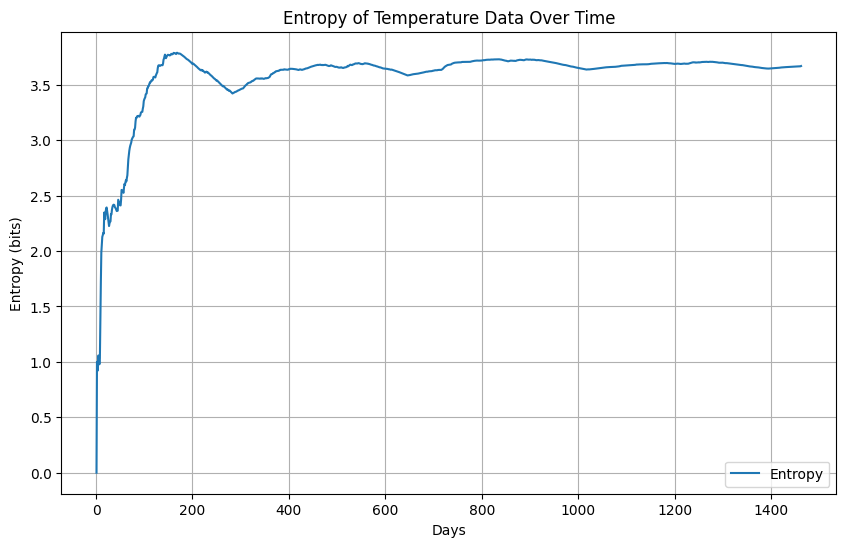
\includegraphics[width=0.5\linewidth]{entropy.png}
    \label{fig:enter-label}
\end{figure}
\end{frame}

\begin{frame}{Result}
The process repeats, recalculating probabilities and entropy at every step, and the results are stored in a list called "entropy values". Finally, the entropy values are plotted against time (days). The x-axis represents the number of days (i.e., how much data has been accumulated), and the y-axis represents the entropy (measured in bits).

At the very beginning (first 50–200 days), the entropy rises sharply. This indicates that the uncertainty in the dataset is increasing rapidly. As more data is introduced, the system is becoming less predictable—likely because more variations in temperature are being captured. After the sharp rise, the entropy curve flattens out and oscillates around a value close to 3.5 bits. This stabilization indicates that the system has reached a point where additional data does not significantly increase uncertainty. In other words, the temperature data has become more predictable, and no new significant randomness is being introduced.
\end{frame}
\begin{frame}{Result}

The plot suggests that the temperature dataset initially had a lot of variability, but as more data was accumulated, the variability reached a limit. This pattern is common in systems where initial observations are more uncertain but then start to follow a more predictable pattern as the dataset grows.
\end{frame}

\section{Exercise3}

\begin{frame}{Exercise 1: Title of the Exercise}
\textbf{Description}

This is the content of Exercise 3.
\end{frame}


\section{Exercise 4: Information Gain Ratio }

\begin{frame}{Information Gain Ratio }
In this exercise we aim to:
\begin{itemize}
    \item Compute the Information Gain Ratio with respect to all the other
variables and select the one that provides more information about X
\end{itemize}
\end{frame}

\begin{frame}{DataSet}
For This exercise we made a dataset which has some features like pageViews, Time on site, age group, and country and our target is purchase, we want to figure out which feature has the most impact on purchases.
\begin{figure}
    \centering
    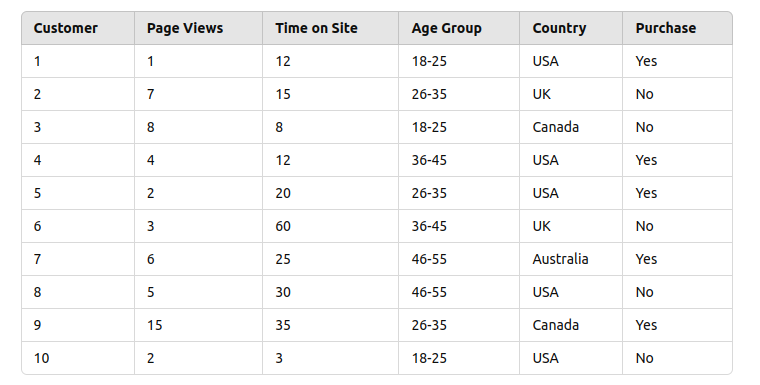
\includegraphics[width=0.7\linewidth]{image.png}
    
    \label{fig:enter-label}
\end{figure}

\end{frame}
\begin{frame}{Calculate Information Gain}
    Our first step is calculate the Entropy of the target variable purchase (yes/no). This will serve as our baseline entropy for evaluating the effect of each feature.

    The Entropy formula is:
    \[
H(X) = -\sum_{i=1}^{n} p(x_i) \log_2{p(x_i)}
\]
Then for each feature in the dataset calculates the Information Gain with respect to the target variable Purchases.

The Information Gain formula is:
\[
IG(Y,X) = H(Y) - H(Y|X)
\]
where:

$H(Y)$is the entropy of the target variable


$H(Y|X)$is the conditional entropy of the target variable given the feature X

\end{frame}



\begin{frame}{Calculate Information Gain}
In this exercise, we use the concept of Information Gain Ratio to determine the most influential factor among the given attributes for predicting a purchase.

Information gain(IG):Measures how much information each feature provides about the purchase, Higher values indicate more informative features and Range: from 0 (no information) to 1 (perfect information)

Gain Raito: Normalizes Information Gain by Split Information, Provides a fairer comparison between features, Higher values indicate better predictive power

\end{frame}

\begin{frame}{Calculation Information Gain}
The next step is to calculate the conditional entropy of the target variable given each of the other features. This measures the remaining uncertainty about the target variable after knowing the value of a feature.

For each feature (like time on site), the conditional entropy is calculated as:
    \[
H(Purchase|Time On Site) = -\sum_{i=1}^{n} p(x_i) . H(purchase|x_i)
\]
where $H(Purchase|X_i)$ is the entropy of the target variable within each group of the feature.


\end{frame}



\begin{frame}{Calculate Information Gain}
The formula for Information Gain Ratio is:
    \[
IGR(Y,X) = \frac{IG(Y,X)} {H(X)}
\]
After calculating the Information Gain Ratio for each feature, selected the feature with the highest value. 
\begin{figure}
    \centering
    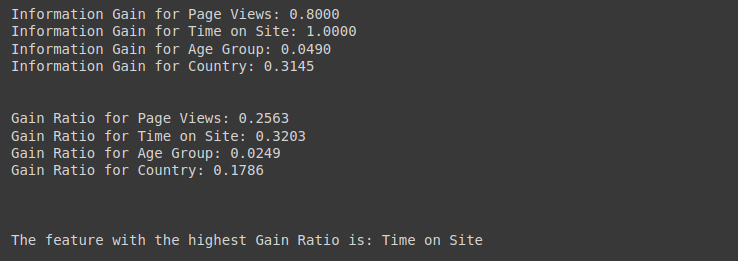
\includegraphics[width=0.7\linewidth]{oh.png}
    \label{fig:enter-label}
\end{figure}
\end{frame}
\begin{frame}{Result}
    The information gain measures how much knowing a feature reduces uncertainty about
the target variable. A high information gain means the feature provides significant
information about the target.we compute The Information Gain Ratio which adjusts the information gain
by accounting for the intrinsic information of the feature itself. Features with more
distinct values (like those with more categories) tend to have higher information gain, so
the Information Gain Ratio helps to normalize this bias.Finally we can the feature which provides the most important information for target variable
\end{frame}

\section{Exercise 5: Kullback-Leibler divergence from empirical distribution}

\begin{frame}{Kullback-Leibler divergence}
	
	In this exercise we try to identify which binomial distribution is the best analytical fit for our sampled distribution.
	
	To do so, we need to introduce the concept of \textbf{Kullback-Leibler divergence}. Kullback-Leibler divergence is a statistical measure that quantifies how much one probability distribution differs from a second, reference probability distribution. KL divergence is closely linked to conditional entropy and information gain, because it measures how much more uncertainty is introduced by using one probability distribution instead of another.
	
	For two probability distributions \(P\) (the observed distribution) and \(Q\) (the analytical fit), the KL divergence from \(Q\) to \(P\) is given by:
	
	\[
	D_{KL}(P || Q) = \sum_{x} P(x) \log \left( \frac{P(x)}{Q(x)} \right)
	\]
	
\end{frame}

\begin{frame}{Observed Distribution}
	Consider the following observed data:
	
	\[
	x_{i} = (0\quad 1\quad 2\quad 3\quad 4\quad 5\quad 6\quad 7\quad 8\quad 9\quad 10)
	\]
	
	\[
	\# \quad observed \quad x_{i} = (1\quad 3\quad 2\quad 8\quad 18\quad 41\quad 47\quad 39\quad 24\quad 8\quad 3)
	\]
	
\end{frame}

\begin{frame}{Divergence from Uniform Distribution}
	
	We compute the KL divergence of the observed distribution from a uniform distribution, to measure how distant the two probability distributions are.
	
	\begin{figure}[h]
		\centering
		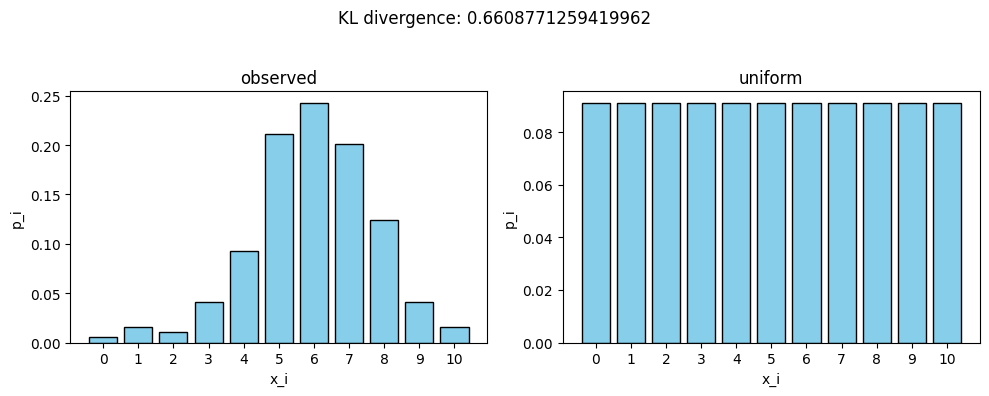
\includegraphics[width=.9\textwidth]{images/ex5/uniform_div.png}
	\end{figure}
	
\end{frame}

\begin{frame}{Search of the optimal Binomial Distribution}
	
	To find the binomial distribution closest to the observed distribution, we compute the KL divergence from each binomial distribution given \(n=11\) independent experiments and probability of success \(p\) ranging between 0 and 1 (step = 0.001).
	
	\begin{figure}[h]
		\centering
		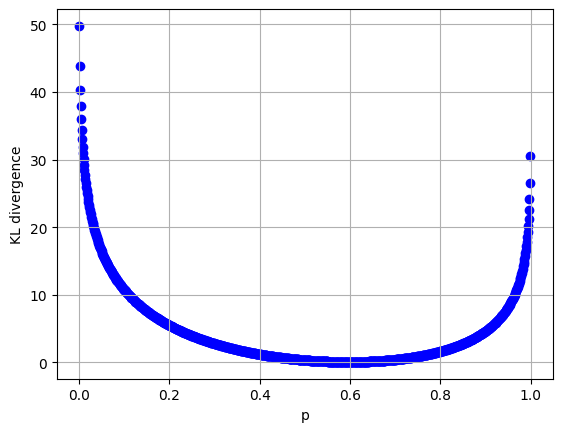
\includegraphics[width=.43\textwidth]{images/ex5/binomial_kl.png}
	\end{figure}
	
\end{frame}

\begin{frame}{Best Binomial Distribution}
	
	By minimizing the KL divergence, we determine that the optimal binomial distribution has a success probability \(p = 0.596\). We can see from the histograms that the 2 distributions are very similar and the KL divergence value has dropped significantly. 
	
	\begin{figure}[h]
		\centering
		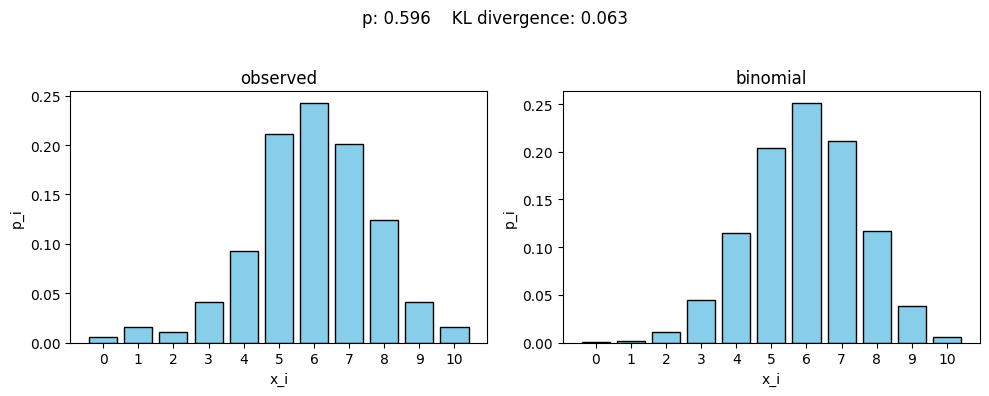
\includegraphics[width=.75\textwidth]{images/ex5/best_binomial.png}
	\end{figure}
	
\end{frame}


\begin{frame}{Conclusion}
	
	We successfully used Kullback-Leibler divergence to identify the binomial distribution that best approximates the observed data, minimizing the error committed. With this approach we can accurately model empirical distributions and also understand the degree of divergence between the observed distributions and their analytical fits.
	
\end{frame}


\section{Exercise 6: Permutation Entropy Analysis}

\begin{frame}{Data Generation and Parameters}
We generated a random data series of length 10,000 using a uniform distribution between 0 and 1:

\[
x = [x_1, x_2, \dots, x_{10000}], \quad x_i \in [0, 1]
\]

The entropy calculation was carried out using:
\begin{itemize}
    \item Sliding window size: \( N_w = 512 \)
    \item Permutation order: \( m = 3 \)
\end{itemize}
\end{frame}

\begin{frame}{Sliding Window and Permutation Entropy}
The data series was divided into overlapping windows of size \( N_w = 512 \). Within each window, we mapped the sequence to a permutation by sorting the indices of the data values.

The permutation entropy for each window was calculated as:

\[
H(\pi) = - \sum P(\pi) \log_2 P(\pi), \quad P(\pi) = \frac{\text{count of permutation } \pi}{\text{total number of permutations in the window}}
\]

The entropy was then normalized:

\[
H' = \frac{H(\pi)}{\log_2(m!)}
\]

where \( H' \) ranges from 0 (fully predictable data) to 1 (completely random data).
\end{frame}

\begin{frame}{Random Data Series Plot}
\begin{figure}[ht]
    \centering
    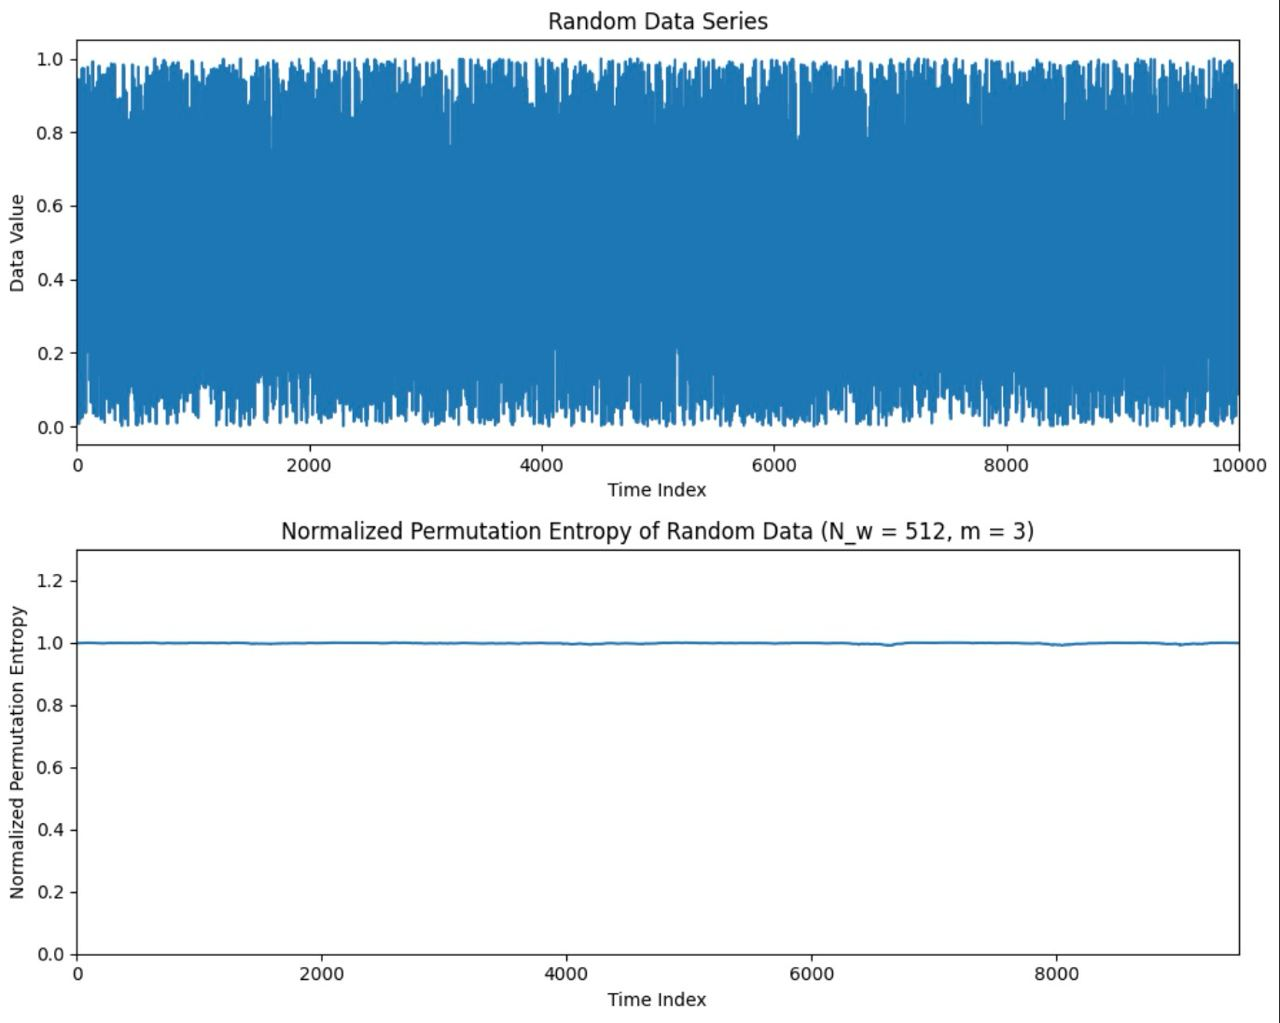
\includegraphics[width=0.5\textwidth]{images/first.jpg}
    \caption{Random data series and corresponding permutation entropy, showing high randomness with entropy near the maximum value.}
\end{figure}
\end{frame}

\begin{frame}{Data Modification: Structured Pattern}
To introduce a structured pattern, the segment between indices \textbf{3000} and \textbf{4000} was partially sorted in chunks of size 20:

\[
x_{i:i+20} = \text{sort}(x_{i:i+20}) \quad \text{for } i \in [3000, 4000]
\]

This reduced the randomness while keeping the mean and variance of the data consistent.
\end{frame}

\begin{frame}{Modified Data Series Plot}
\begin{figure}[ht]
    \centering
    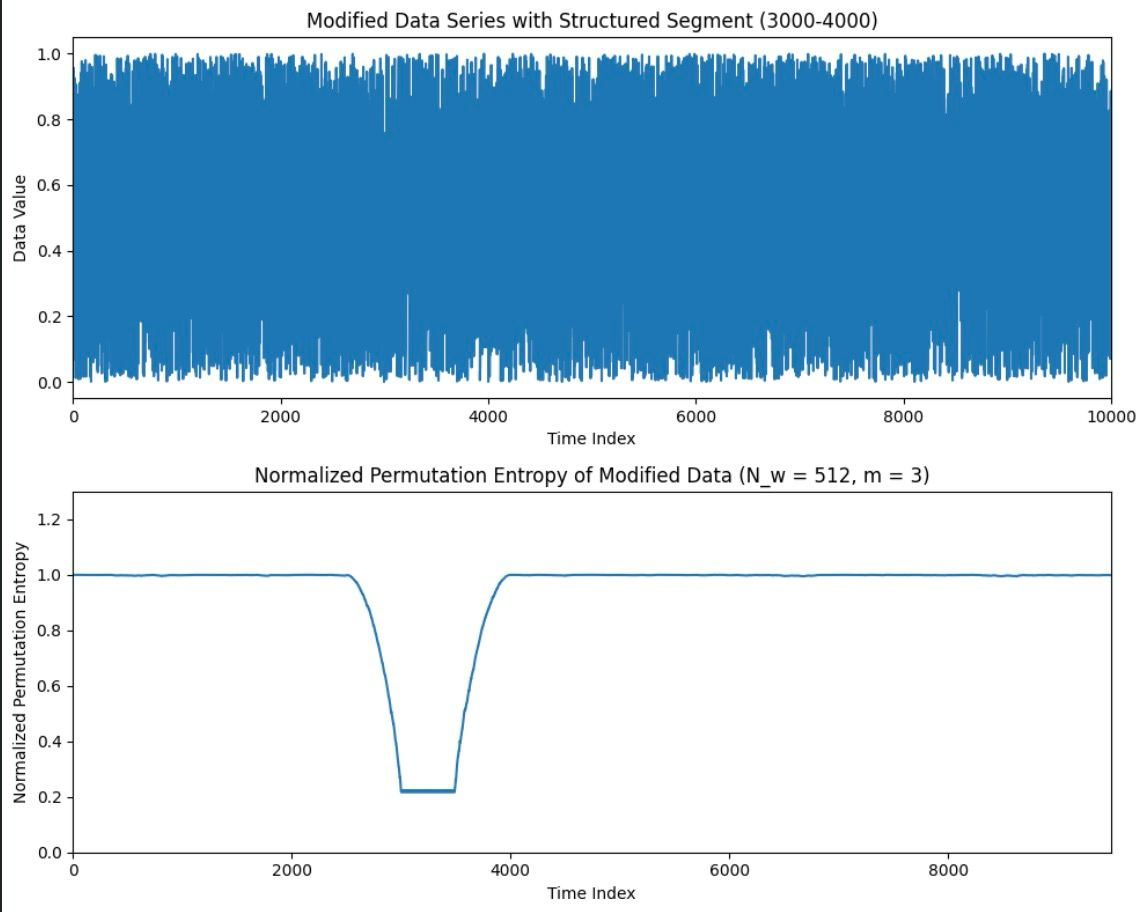
\includegraphics[width=0.5\textwidth]{images/second.jpg}
    \caption{Modified data series with a structured segment (indices 3000 to 4000). The entropy decreases, indicating reduced randomness.}
\end{figure}
\end{frame}

\begin{frame}{Results and Analysis}
For the \textbf{random data series}, the entropy remained close to the theoretical maximum:

\[
H_{\max} = \log_2(m!) = \log_2(6) \approx 2.585
\]

The normalized permutation entropy approached \textbf{1}, implying a high degree of randomness. 

After modifying the segment between indices \textbf{3000} and \textbf{4000}, the entropy dropped due to the partial sorting, indicating reduced randomness in that region:

\[
H' < 1 \quad \text{for the modified region}
\]
\end{frame}

\begin{frame}{Conclusion}
The \textbf{permutation entropy} effectively captured changes in the time series complexity. The random data exhibited entropy near the theoretical maximum, while the structured segment showed a decrease in entropy, indicating the presence of a pattern.

Permutation entropy is useful for detecting complexity changes and can be applied in anomaly detection in more complex datasets.
\end{frame}


\section{Exercise 7}

\begin{frame}{Information Gain Ratio and Classifiers}
\textbf{Description}

In this exercise we create a classifier, implemented as a decision tree,
using the principle of maximum information gain ratio. A decision tree classifier is an algorithm that classifies a vector of feaures using the following iterative steps for each node of the tree

\begin{itemize}
	
	\item If all the vector in the training set belong to the same class
	
	\item For each node, it analyzes a single feature and moves on the next node based on the result of the analysis. If the feature has limited number of possibile values, a branch is created for each value. If the feature has a numerical value, the value is compared with a threshold and a branch is created for each result of the comparison
	
	\item If all the vector in the training set 



\end{itemize}

analyzing a single feature in each node and moving on the next node based on the result of the analysis, until a leaf

This principle states that the features

\end{frame}

The principle of maximum 


\begin{frame}
	
\end{frame}



\backmatter
\end{document}
